% vim:set et sw=2 ts=4 tw=72:
\chapter{Evaluation}

In June 2017, I conducted a study to quantitatively and qualitatively
evaluate the effectiveness of the visualizations and summaries presented
in \tool{} to the DAG-bed visualizations found in Gitk and the git
command-line. The study was performed in a controlled environment
running Ubuntu 14.04. Participants were allowed to use Gitk and the git
command-line tools for these tasks, I will refer to both tools as Gitk,
when working with DAG-based visualizations and summarizations. I
considered allowing participants to use any of the free tools for Linux
suggested on the git
website\footnote{\url{https://git-scm.com/download/gui/linux}}, but
after attempting to use them, I found that none were able to operate on
repositories that were as large as the Linux repository. \tool{} was
used for evaluating the \mt{-based} visualizations.

The study has two primary goals; first determining if the DAG-based
visualization is sufficient for conceptual understanding, second
comparing \tool and Gitk to determine which is more capable of providing
users with a summarization of various metrics involved with integrating
a commit into the repository.

The first part of the study are conceptual questions. These questions
are designed to test the conceptual understanding drawn from the DAG
visualization. The participants will be working with Gitk to answer
RQ\ref{RQ1}. More details about this part of the study are discussed in
Section~\ref{sec:conceptual_study}. The second part of the study involve
summarizing information about the commits that are related to a given
commit. The participants work with both Gitk and \tool{} in this part of
the study. More details are discussing in
Section~\ref{sec:summarization_study}. A third part asks for the
opinions of the participants regarding their preferences, and why they
felt that way.

\section{Commit Selection}\label{sec:commit_selection}

Two commits are used in both the conceptual study and summarization
study, with the goal of determining how well the DAG and \mt{}
visualizations scale between merges integrating varying numbers of
commits. The order that the two commits are presented to each
participant is randomized. I analyzed 15096 merge-trees from the
database that were candidates for the study, from April 16th 2005 to
October 14th 2014, corresponding to Linux releases 2.6.12-rc3 to
3.17-rc1. A merge-tree could only be selected if it was not a foxtrot,
and had correctly been identified. 25\% of the trees contain at most a
single repository event, not including the root, while 50\% of the trees
contain at most seven nodes. 75\% of the trees contain at least 51
nodes, and the largest tree contains 7217 nodes. 8031 trees contained at
least seven nodes, of these only 593 contained at least a single
internal merge node. Trivially, trees with a single node cannot have any
internal merge nodes. Of the 624 trees with seven non-root node, only
135 contained at least one inner node. Using this information, I chose a
random tree from the 2008 trees in the first quartile, which merges a
single commit into the master branch. These trees are trivial, but
appear frequently in the repository. The second tree was chosen randomly
from trees in the second quartile. These trees contain seven nodes, and
to increase the complexity of the tree, I required that the tree contain
at least one internal merge node.

Once the trees were selected, I had to select a commit from the tree.
Selecting a commit from the small tree was trivial, there was only a
single node to choose. From the medium-sized tree, I used a script to
select a commit randomly. The commits selected from the small tree and
medium tree were \emph{a3c1239eb59c0a907f8be5587d42e950f44543f8} and
\emph{cdbdd1676a5379f1d5cbd4d476f5e349f445befe} respectively. Commit 1,
the commit from the small tree is visualized in
Figure~\ref{fig:commit_1_visualization}, showing the DAG visualization
by Gitk and \rt{} tree visualization in Linvis. The same is
shown for commit 2 in Figure~\ref{fig:commit_2_visualization}.

\begin{figure}[htpb]
  \centering
  \begin{tabular}{cc}
    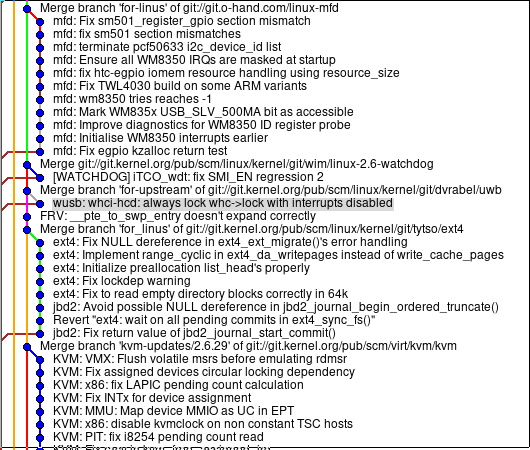
\includegraphics[height=4.5cm]{Figures/evaluation/commit1_gitk.png} &
    
\includegraphics[height=4.5cm]{Figures/evaluation/commit1_linvis.pdf}
  \end{tabular}
  \caption{The visualizations of commit 1 by Gitk and Linvis
    respectively.}
  \label{fig:commit_1_visualization}
\end{figure}

\begin{figure}[htpb]
  \centering
  \begin{tabular}{cc}
    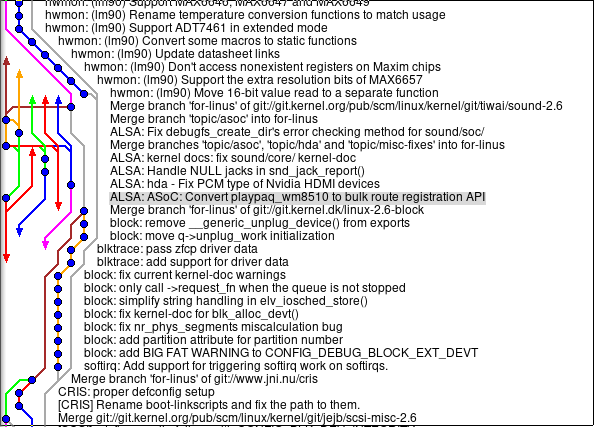
\includegraphics[height=4.5cm]{Figures/evaluation/commit2_gitk.png} &
    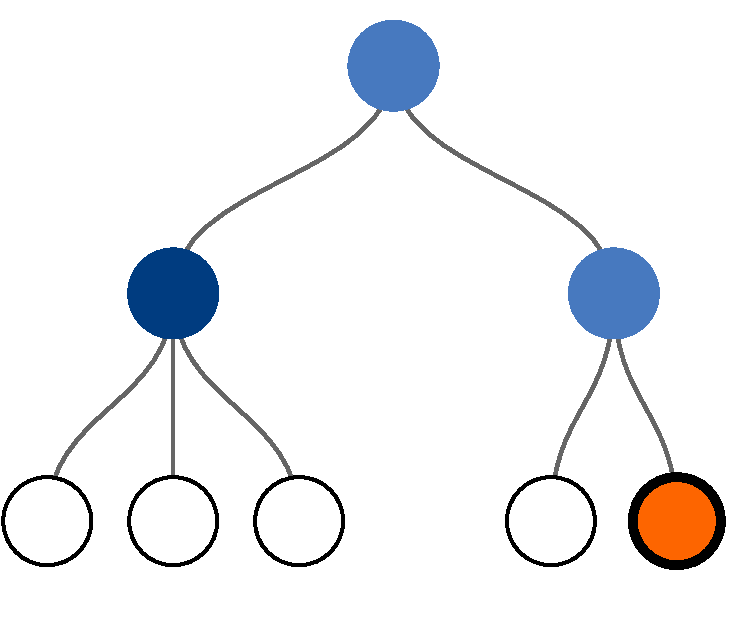
\includegraphics[height=4.5cm]{Figures/evaluation/commit2_linvis.pdf}
  \end{tabular}
  \caption{The visualizations of commit 2 by Gitk and Linvis
    respectively.}
  \label{fig:commit_2_visualization}
\end{figure}
